\chapter{需求建模 }
\section{数据流图}
\subsection{顶层数据流图}

\begin{figure}[ht]
\centering
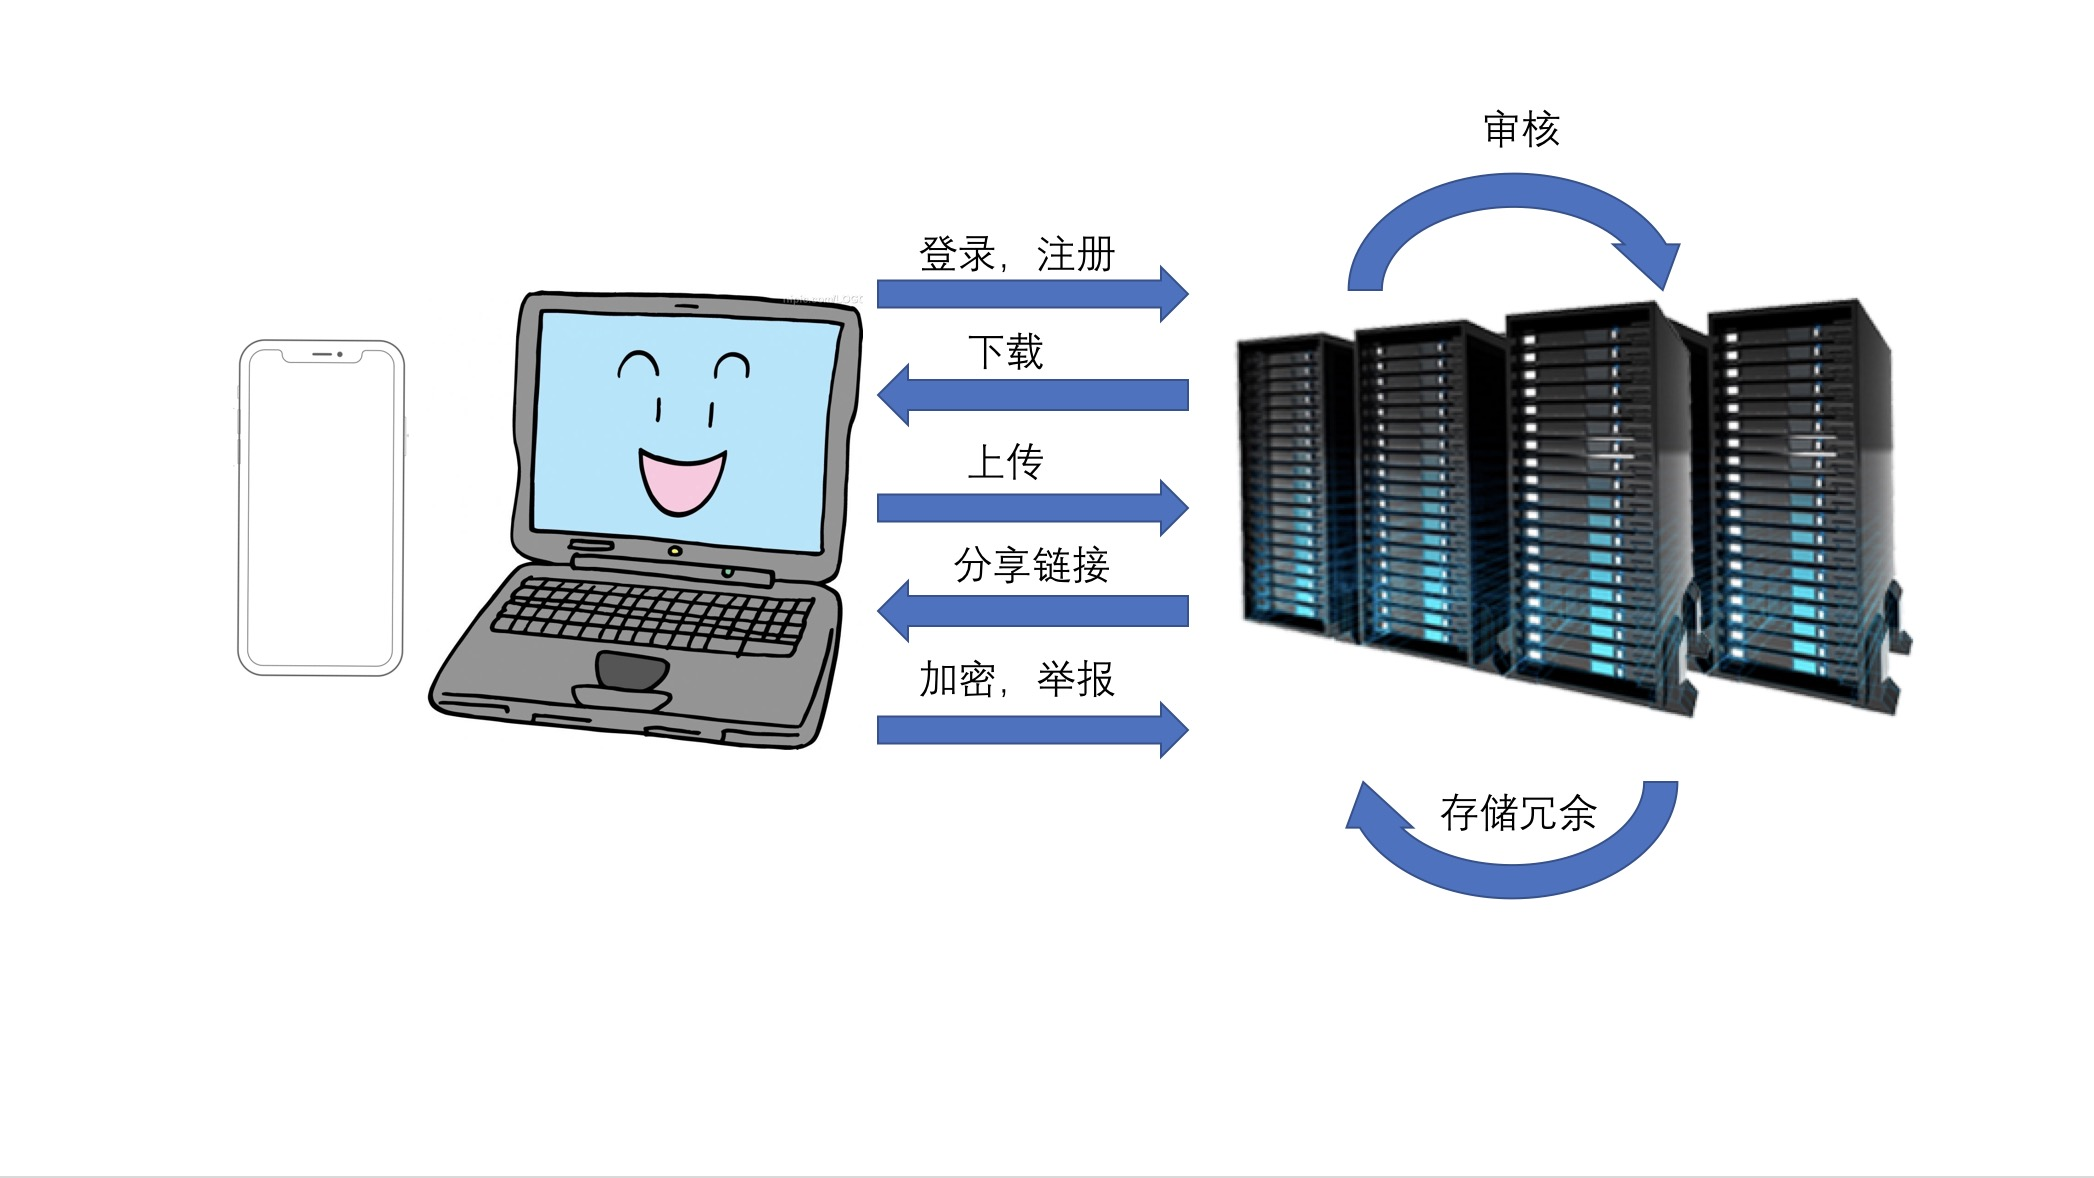
\includegraphics[width=16cm]{top.png}
\caption{顶层数据流图}\label{fig:noted-figure}
\end{figure}

\subsection{层数据流图}

在这里画出0层数据流图
 
\subsection{层数据流图}
<Draw the Level-1 DFD here>

在这里画出1层数据流图

\section{数据字典}
\subsection{数据流说明}
\subsubsection{用户信息}
来源:用户

简述:用户的基本个人信息

去向:服务器

\subsubsection{上传文件}
来源:用户

简述:用户上传到云盘中的文件

去向:服务器

\subsubsection{下载文件}
来源:服务器

简述:通过链接下载的文件

去向:用户/游客

\subsection{数据存储说明}
\subsubsection{用户信息数据表}
描述:保存每个用户相关信息的数据表

来源:用户创建,修改操作

去处:身份验证系统,指令管理系统

组成:用户名+密码

排序方式:用户名的字典序

\subsubsection{上传文件数据表}
描述:保存每个用户云盘文件的数据表

来源:用户上传的文件

去处:数据库系统

组成:用户信息+目的路径+二进制文件

排序方式:用户信息, 文件路径的字典序

\subsubsection{下载文件数据表}
描述:从云盘中下载文件的数据表

来源:数据库系统

去处:用户或游客

组成:文件链接+二进制文件

排序方式:文件名的字典序

\subsection{加工说明}
\subsubsection{验证信息合法性}
输入:用户名密码

输出:登录/注册结果

操作:对于登录请求,判断用户名是否存在。对于注册请求,判断用户名是否合法、是否已经存在、密码是否过于简单。

\subsubsection{计算密码散列值}
输入:用户名密码

输出:用户名和密码的散列值

操作:使用sha256散列值算法,通过密码(原文),用户名和随机数计算密码的散列值。

\subsubsection{权限控制}
输入:管理云端文件系统的指令

输出:返回结果(是否成功)

操作:根据用户的身份信息和文件类型,判断用户是否有权限及该指令是否合法